% vim:ts=4:sw=4
%
% Copyright (c) 2008-2009 solvethis
% Copyright (c) 2010-2015 Casper Ti. Vector
% Public domain.
%
% 使用前请先仔细阅读 pkuthss 和 biblatex-caspervector 的文档,
% 特别是其中的 FAQ 部分和用红色强调的部分。
% 两者可在终端/命令提示符中用
%   texdoc pkuthss
%   texdoc biblatex-caspervector
% 调出。

% 采用了自定义的(包括大小写不同于原文件的)字体文件名,
% 并改动 ctex.cfg 等配置文件的用户请自行加入 nofonts 选项;
% 其它用户不用加入 nofonts 选项,加入之后反而会产生错误。
%
% 图书馆要求电子版论文的目录必须为黑色,
% 且某些教务要求打印版论文的文字部分为纯黑色而非灰度打印,
% 【因此最终打印和提交论文前,请将“colorlinks”改为“nocolorlinks”。】
\documentclass[UTF8, colorlinks, oneside]{pkuthss}

% 使用 biblatex 排版参考文献,并规定其格式。
%
% 如果无法使用 biber,可以把“backend = biber”改为“backend = bibtex”,
% 并改用 bibtex 产生参考文献,详见 pkuthss 的文档。
% 使用 biber 时,请去掉所有的 sorting 选项,否则会出错。
%
% 默认按照引用顺序排序(“sorting = none”),详见 biblatex-caspervector 的文档
% (因为是默认设置所以其实不用写,不过出于完备性的考虑仍然在这里列出)。
% 若需要按照英文文献在前,中文文献在后排序,请设置“sorting = ecnty”;
% 若需要按照中文文献在前,英文文献在后排序,请设置“sorting = centy”。
\usepackage[backend = biber, style = caspervector, utf8, sorting = none]{biblatex}
% 提供近似于学校所要求的 Times New Roman / Arial 的字体。
\usepackage[defaultsups]{newtxtext}
\usepackage{newtxmath}
% 产生 originauth.tex 里的 \square。
\usepackage{amssymb}
\usepackage{amsmath}
\usepackage{graphicx}
\usepackage{listings}
\usepackage[usenames,dvipsnames]{color}
\usepackage{xcolor}
% 按学校要求设定参考文献列表中的条目之内及之间的距离。
\setlength{\bibitemsep}{3bp}
% 对于 linespread 值的计算过程有兴趣的同学可以参考 pkuthss-extra.sty。
\renewcommand*{\bibfont}{\zihao{5}\linespread{1.27}\selectfont}

% 设定文档的基本信息。
\pkuthssinfo{
	cthesisname = {本科生毕业论文}, ethesisname = {Undergraduate Thesis},
	ctitle = {API迁移问题上的程序变换语言设计与实现}, etitle = {A Safe Transformation Language for Code Adaptation between APIs},
	cauthor = {汪成龙},
	eauthor = {Chenglong Wang},
	studentid = {1100012785},
	date = {2015.05.21},
	school = {信息科学技术学院},
	cmajor = {计算机专业}, emajor = {Computer Science},
	direction = {程序语言},
	cmentor = {熊英飞}, ementor = {Prof.\ Yingfei Xiong},
	ckeywords = {程序语言,程序变换}, ekeywords = {Programming languages, Program transformation}
}
% 载入参考文献数据库(注意不要省略“.bib”)。
\addbibresource{thesis.bib}

% 普通用户可删除此段。
\usepackage{color}
\def\pkuthssffaq{%
	\emph{\textcolor{red}{pkuthss 文档模版最常见问题:}}

	在最终打印和提交论文之前,
	请将 pkuthss 文档类选项中的 %
	\texttt{colorlinks} 改为 \texttt{nocolorlinks},
	因为图书馆要求电子版论文的目录必须为黑色,
	且某些教务要求打印版论文的文字部分为纯黑色而非灰度打印。

	\texttt{\string\cite}、\texttt{\string\parencite} %
	和 \texttt{\string\supercite} 三个命令分别产生%
	未格式化的、带方括号的和上标且带方括号的引用标记:%
	\cite{test-en},\parencite{test-zh}、\supercite{test-en, test-zh}。

	若要避免章末空白页,请在调用 pkuthss 文档类时加入 \texttt{openany} 选项。

	如果编译时不出参考文献,
	请参考 \texttt{texdoc pkuthss}“问题及其解决”一章
	“其它可能存在的问题”一节中关于 biber 的说明。
}

\newcommand{\code}[1]{\texttt{\footnotesize #1}}
\newcommand{\flyingbox}[1]{\begin{flushleft}\fbox{{#1}}\end{flushleft}}
\newcommand{\todo}[1]{{\bf \{TODO: {#1}\}}}
\newcommand{\figref}[1]{{图.\ref{#1}}}
\newtheorem{theorem}{Theorem}
\newtheorem{lemma}{Lemma}
\newtheorem{definition}{Definition}
\newtheorem{property}{Property}
\usepackage[all,cmtip]{xy}

\newsavebox{\fmbox}
\newenvironment{fmpage}[1]
{\begin{lrbox}{\fmbox}\begin{minipage}{#1}}
{\end{minipage}\end{lrbox}\fbox{\usebox{\fmbox}}}

\newenvironment{smpage}[1]
{\begin{lrbox}{\fmbox}\begin{minipage}{#1}}
{\end{minipage}\end{lrbox}\usebox{\fmbox}}

\newcommand{\textcd}[1]{\text{\scriptsize\BeraMonottfamily{#1}}}

\lstdefinestyle{patl}{ % Define a style for your code snippet, multiple definitions can be made if, for example, you wish to insert multiple code snippets using different programming languages into one document
%backgroundcolor=\color{highlight}, % Set the background color for the snippet - useful for highlighting
basicstyle=\footnotesize\ttfamily, % The default font size and style of the code
breakatwhitespace=false, % If true, only allows line breaks at white space
breaklines=true, % Automatic line breaking (prevents code from protruding outside the box)
captionpos=b, % Sets the caption position: b for bottom; t for top
commentstyle=\usefont{T1}{pcr}{m}{sl}\color{DarkGreen}, % Style of comments within the code - dark green courier font
deletekeywords={}, % If you want to delete any keywords from the current language separate them by commas
%escapeinside={\%}, % This allows you to escape to LaTeX using the character in the bracket
firstnumber=1, % Line numbers begin at line 1
frame=none, % Frame around the code box, value can be: none, leftline, topline, bottomline, lines, single, shadowbox
frameround=tttt, % Rounds the corners of the frame for the top left, top right, bottom left and bottom right positions
keywordstyle={[1]\color{blue!90!black}},
keywordstyle={[3]\color{red!80!orange}},
morekeywords={}, % Add any functions no included by default here separated by commas
numbers=left, % Location of line numbers, can take the values of: none, left, right
numbersep=3pt, % Distance of line numbers from the code box
numberstyle=\tiny\color{Gray}, % Style used for line numbers
rulecolor=\color{black}, % Frame border color
showstringspaces=false, % Don't put marks in string spaces
showtabs=false, % Display tabs in the code as lines
stepnumber=1, % The step distance between line numbers, i.e. how often will lines be numbered
tabsize=2, % Number of spaces per tab in the code
}
\lstset{escapeinside={@}{@}}

\lstdefinestyle{java}{ % Define a style for your code snippet, multiple definitions can be made if, for example, you wish to insert multiple code snippets using different programming languages into one document
%backgroundcolor=\color{highlight}, % Set the background color for the snippet - useful for highlighting
basicstyle=\footnotesize\ttfamily, % The default font size and style of the code
breakatwhitespace=false, % If true, only allows line breaks at white space
breaklines=true, % Automatic line breaking (prevents code from protruding outside the box)
captionpos=b, % Sets the caption position: b for bottom; t for top
commentstyle=\usefont{T1}{pcr}{m}{sl}\color{DarkGreen}, % Style of comments within the code - dark green courier font
deletekeywords={}, % If you want to delete any keywords from the current language separate them by commas
%escapeinside={\%}, % This allows you to escape to LaTeX using the character in the bracket
firstnumber=1, % Line numbers begin at line 1
frame=none, % Frame around the code box, value can be: none, leftline, topline, bottomline, lines, single, shadowbox
frameround=tttt, % Rounds the corners of the frame for the top left, top right, bottom left and bottom right positions
keywordstyle={[1]\color{blue!90!black}},
keywordstyle={[3]\color{red!80!orange}},
morekeywords={}, % Add any functions no included by default here separated by commas
numbers=left, % Location of line numbers, can take the values of: none, left, right
numbersep=3pt, % Distance of line numbers from the code box
numberstyle=\tiny\color{Gray}, % Style used for line numbers
rulecolor=\color{black}, % Frame border color
showstringspaces=false, % Don't put marks in string spaces
showtabs=false, % Display tabs in the code as lines
stepnumber=1, % The step distance between line numbers, i.e. how often will lines be numbered
tabsize=2, % Number of spaces per tab in the code
}
\lstset{escapeinside={@}{@}}

\begin{document}
	% 以下为正文之前的部分,默认不进行章节编号。
	\frontmatter
	% 此后到下一 \pagestyle 命令之前不排版页眉或页脚。
	\pagestyle{empty}

	% 自动生成标题页。
	\maketitle
	% 版权声明。
	% vim:ts=4:sw=4
%
% Copyright (c) 2008-2009 solvethis
% Copyright (c) 2010-2015 Casper Ti. Vector
% All rights reserved.
%
% Redistribution and use in source and binary forms, with or without
% modification, are permitted provided that the following conditions are
% met:
%
% * Redistributions of source code must retain the above copyright notice,
%   this list of conditions and the following disclaimer.
% * Redistributions in binary form must reproduce the above copyright
%   notice, this list of conditions and the following disclaimer in the
%   documentation and/or other materials provided with the distribution.
% * Neither the name of Peking University nor the names of its contributors
%   may be used to endorse or promote products derived from this software
%   without specific prior written permission.
%
% THIS SOFTWARE IS PROVIDED BY THE COPYRIGHT HOLDERS AND CONTRIBUTORS "AS
% IS" AND ANY EXPRESS OR IMPLIED WARRANTIES, INCLUDING, BUT NOT LIMITED TO,
% THE IMPLIED WARRANTIES OF MERCHANTABILITY AND FITNESS FOR A PARTICULAR
% PURPOSE ARE DISCLAIMED. IN NO EVENT SHALL THE COPYRIGHT HOLDER OR
% CONTRIBUTORS BE LIABLE FOR ANY DIRECT, INDIRECT, INCIDENTAL, SPECIAL,
% EXEMPLARY, OR CONSEQUENTIAL DAMAGES (INCLUDING, BUT NOT LIMITED TO,
% PROCUREMENT OF SUBSTITUTE GOODS OR SERVICES; LOSS OF USE, DATA, OR
% PROFITS; OR BUSINESS INTERRUPTION) HOWEVER CAUSED AND ON ANY THEORY OF
% LIABILITY, WHETHER IN CONTRACT, STRICT LIABILITY, OR TORT (INCLUDING
% NEGLIGENCE OR OTHERWISE) ARISING IN ANY WAY OUT OF THE USE OF THIS
% SOFTWARE, EVEN IF ADVISED OF THE POSSIBILITY OF SUCH DAMAGE.

\chapter*{版权声明}
\thispagestyle{empty}

任何收存和保管本论文各种版本的单位和个人,
未经本论文作者同意,不得将本论文转借他人,
亦不得随意复制、抄录、拍照或以任何方式传播。
否则一旦引起有碍作者著作权之问题,将可能承担法律责任。

% 若需排版二维码,请将二维码图片重命名为“barcode”,
% 转为合适的图片格式,并放在当前目录下,然后去掉下面 3 行的注释。
%\vfill\noindent
%\includegraphics[height = 5em]{barcode}



	% 此后到下一 \pagestyle 命令之前正常排版页眉和页脚。
	\cleardoublepage
	\pagestyle{plain}
	% 重置页码计数器,用大写罗马数字排版此部分页码。
	\setcounter{page}{0}
	\pagenumbering{Roman}

	% 中英文摘要。
	% vim:ts=4:sw=4
%!TEX root=../thesis.tex
% Copyright (c) 2014 Casper Ti. Vector
% Public domain.

\begin{cabstract}
	现代软件的开发离不开对于API的依赖,API的版本升级问题,以及对于API需求变化带来的API迁移问题就成为了软件维护的一个重要问题。在大规模的软件开发过程中,手动维护会极大的增加软件的维护成本,同时较高的错误率也导致了其他维护问题的产生。因此,能够快速的开发一个能够保证程序变换正确性的自动化工具就成为了软件维护者的梦想。

	然而,API之间复杂的映射,尤其是多对多的API调用映射关系,让自动转换工具的开发变得尤为困难。本文设计了一种领域特定语言(Domain Specific Language)来解决因API问题而进行程序改写的问题,通过语言机制来保证了API迁移过程中的程序变换的正确性,同时提供了用户友好的映射规则定义接口。本文定义了该程序变换语言的表里语义:表语义为用户书写转换规则过程中对于API规则的理解,而里语义则是转换规则在程序变换过程中的作用法则,并通过程序分析的手段来自动分析API转换规则在用户程序中的依赖关系,让程序的表里语义能够在实际转换过程中起到等同的作用,以此来保证变换过程在符合语言使用者理解的条件下自动推广到复杂的显示情况中。
\end{cabstract}

\begin{eabstract}
	Modern software development can not progress without the use of APIs, and this makes incompatible API update or API switching become an important but tough task for software maintainers. It is not feasible for programmers to manually update these programs between the APIs, as errors are likely to appear with manual effort, which even increases the cost of software maintenance. Thus it is desirable to have automatic program transformation tools to support the program transformation process that can maintaining the safety of the transformation process.

	To make the transformation tool programming easier, we designed a domain specific language PATL, which providing safe checks in the language semantics with user-friendly interface. In the language design, we provide an external semantics, which enables users to understand the rules they write easily, as well as an internal semantics for the actual transformation of user programs that can handle complex program transformation cases. The magic between the two semantics is the design of an analysis system which support semantic-preserving program rewriting before adaptation, which actually achieves the goals to enable users to transform complex programs with their simple rules written with the understanding of the external semantics.
\end{eabstract}


	% 自动生成目录。
	\tableofcontents

	% 以下为正文部分,默认要进行章节编号。
	\mainmatter
	% 序言。
	% vim:ts=4:sw=4
% Copyright (c) 2014 Casper Ti. Vector
% Public domain.
%!TEX root=../thesis.tex

\specialchap{序言}
% 中文测试文字。
现代的程序开发过程大量的依赖着对于API(Application Programming Interfaces,应用程序接口)的使用,因而在程序中进行API的替换也成为了程序开发过程以及软件维护过程中开发者的一项重要工作。其中,程序中的API改写主要可以分为以下两个类别。第一类是API的升级:当一个API推出的新版接口并不兼容旧版API接口时,使用旧版API的用户程序就需要进行改写来满足对于新API的使用。另一类则是API的切换,这一类情况常常出现在用户希望将原有的应用程序迁移到另一个平台上(例如从Android到IOS的程序切换),或是因为对于API性能以及维护功能上的其他需求而要求将原有的API切换到另一个API集合中去。在以上描述的这两种API更替场景中,我们需要将使用$API_1$的程序变换为使用$API_2$的程序,而$API_1$与$API_2$之间具有同构性,这样的替换也即相同功能之间的不同接口替换。然而,这样的程序变换并不容易。当用户手动进行这样的程序转换时,由于并非所有用户都是API的专家,他们并不能够全盘掌握两个API之间的映射关系,以及难以顾及到不同转换之间的交叉问题,手工的转换带来的结果就常常是错漏连篇的新程序,这带来结果就是更加高昂的软件维护成本和更多的人力资源消耗。

既然对于API升级的程序改写如此重要而又如此困难,让API发布者提供一个自动的程序转换工具就成为了帮助客户端程序员(即使用API的用户程序员)进行程序升级的一大利器:当API进行更新的时候,API发布者在发布API库的时候同时提供了一个用户升级工具来帮助客户进行程序升级,用户只需要让工具自动的将原有的程序进行改写就成为了使用新API的程序。让API提供者开发这样的转换工具具有相当的好处:一方面,作为API的专家,他具有更加丰富的API映射关系的知识,他能够处理还API之间的多方面映射关系,而另一方面,这样工具的开发是独立于用户程序的,一次开发就能够让广大用户都可以进行程序的升级,可以广泛的解决用户的需求问题。这样的工具例子有1)微软为了推广自己的.Net平台,提供了Visual Basic到Visual Basic.Net的程序转换工具,2)RIM提供了一个从Android到Blackberry的平台迁移工具,让使用Android API的程序能够自动改写为使用Blackberry的工具,从而可以让转换后的程序在Blackberry上运行而不需更多的工作。

然后,开发这样的Source-to-source自动转换工具并不容易。从转换工具的市场上来看,只有极小的一部分API拥有了这样的自动转换工具来完成程序的改写工作,其中一个重要的原因就是这些API间的程序自动转换工具常常会引入一些新的错误,或是在具体的程序环境中并不能完全按照API开发者的意图进行程序之间的改写。其中一个典型的例子就是Python 2to3.script工具,这个工具是设计来将使用python 2.x版本的程序升级为使用python 3.x版本的程序。虽然这个升级脚本能够在一定程度上完成对于python API的升级工作,但在升级过程中也引入了较多的错误,在有Pilgrim与Willison的案例研究\cite{python}中,2to3.script会导致包括类型错误在内的很多程序错误。从另一方面来看,程序变换开发的困难源自于专业开发环境的支持。由于并非所有的API开发者都能够熟悉程序语言的修改操作,让他们从底层开始实现这样的转换工具就显得困难重重。

事实上,为了解决程序变换的难题,程序语言社区设计出了很多的程序变换语言\cite{twinning}\cite{stratego}\cite{txl}。这些语言通过高层次的抽象来帮助使用者避开了底层开发中容易产生的错误,例如转换语言中能够保证程序变换前后不会产生语法错误,同时能够帮助开发者更好的描述自己需要表达的转换对象。然而对于API迁移这样一个特定场景的问题,这些变换语言的设计就显出了明显的不足,主要体现在以下几个方面:
\begin{itemize}
\item API变换过程中的类型安全并没有得到保证:这些通用的程序变换语言由于广泛的解决了多类的程序变换问题,类型安全就显得难以控制,而在较为单一的API升级问题中,变换对象保持在了statement以及expression层次上,类型的正确性就变得可控同时具有高层次的操作性。
\item API之间的映射没有得到高层次的抽象,因而这些转换仍然需要较多对于用户context的明确指定。由于API转换工具开发者需要能够在未知用户程序环境的情况下完成映射规则的指定,复杂的context就难以得到实现。
\item API升级之中多对多的API映射没有得到良好的支持:API之间的多对多问题涉及到了程序之间的环境分析问题以及转换语句之间的依赖关系问题,而大多数变换语言都是从语形上进行的转换,这样的转换就忽略了转换对象在运行时候的以来关系以及对应关系,从而导致了变换过程的实际语义遭到了违反。
\end{itemize}

我们接下来通过几个实际的例子来描述API之间程序改写中的常见问题。
\paragraph{类型安全问题} 类型安全问题主要体现在程序迁移前是类型正确的而改写之后出现了类型错误,举例如下。(该案例来自\cite{swing2swt})

在Java图形界面编程API Swing到SWT的升级过程中,Swing在创建一个窗口时需要首先创建一个Container来存放窗口中的内容,SWT也同理需要创建一个对应的Composite类来进行存放。(类图见\figref{swing2swtfig})因此在升级过程就就有了这样的两条对应关系(此处的规则只是简单的描述了API之间的映射关系,其中的$\pi_1$可以读作“将\code{Container}类的构造函数映射到\code{Composite}的构造函数,其中\code{Composite}的构造函数参数为\code{new Shell()}以及0”,第二条规则则是将\code{JList}类映射到\code{List}类,并将其构造函数进行对应的替换。):
\[
\begin{array}{ll}
	\pi_1=\code{new Container() ->> new Composite(new Shell(),0)}\\
	\pi_2=\code{new JList() ->> new List()}
\end{array}
\]
\begin{figure}[ht]
\centering
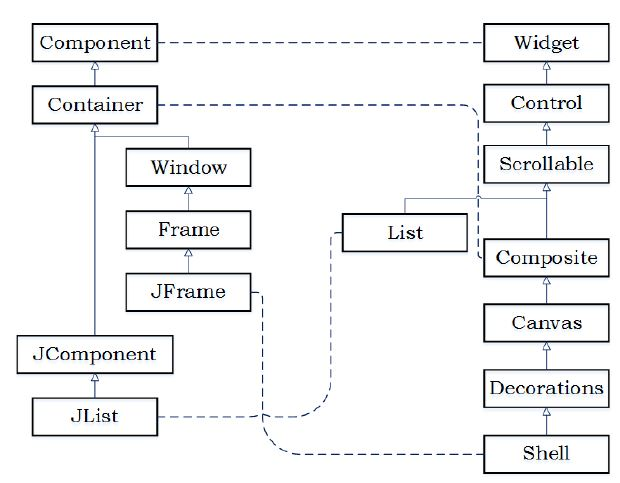
\includegraphics[width=200pt]{fig//swing2swt_class.JPG}
\caption{Swing(图左)到SWT(图右)之间的类图对应关系,其中虚线箭头表示两个API之间的类映射,实线箭头表示同一API中类的继承关系(往下为父类)}
\label{swing2swtfig}
\end{figure}
在这样的转换规则下,用于转换如下用户程序时就会出现类型的错误。
\[
\code{JList list = new Container();} \longrightarrow \code{List list = new Composite(new Shell(), 0);}
\]
其原因在于在\figref{swing2swtfig}中,Swing类型中的JList是Container的父类,因而左部满足子类关系而右部的List不再是Composite的子类,因而转换之前的类型是正确的,而转换之后就会导致类型错误的出现。

\paragraph{API之间多对多的映射问题}
比起前面所提到的类型问题,程序变换中更复杂的多对多问题更为引人注目。API之间多对多映射带来的主要问题则是用户程序上下文之间的不一致性,这样的问题并不像类型错误那样能够通过静态检查就能够得到并修复,而复杂的runtime错误让这类问题更容易隐藏。

在这里我们先简单使用程序匹配语言SmPL\cite{spatch}的语法来展示变换的规则。
\begin{center}
\begin{smpage}{0.25\columnwidth}
\begin{lstlisting}[style=patl]
(a:A->B) {
	- a.x();
	- a.y();
	+ a.z();
}
\end{lstlisting}
\end{smpage}
\end{center}
这一条规则就代表了一组API到另一组API之间的映射,元变量定义部分的\code{a:A->A}就代表了元变量在原来的API集合中类型为A,在新的API集合中类型为B,而这条规则表示了“每当遇到一个类型为A的变量a连续调用了a.x()与a.y()两个方法,我们就删除这两条语句,并用a.z()这样的一条语句来进行替换。”

假设我们现在的转换空间具有如下两条规则:
\begin{center}
\begin{smpage}{0.25\columnwidth}
\begin{lstlisting}[style=patl,frame=none]
(a:A->A) {
  - a.y();
  - a.x(); 
  + a.n(); 
}
\end{lstlisting}
~~~~{\small Rule-1}
\end{smpage}
\qquad\quad
\begin{smpage}{0.35\columnwidth}
\begin{lstlisting}[style=patl,frame=none]
(a:A->A,b:int->int) {
  - b = a.z();
  - a.x();
  + b = a.m(); 
}
\end{lstlisting}
~~~~{\small Rule-2}
\end{smpage}
\end{center}
让我们来考虑如下几种实际的转换类别来分析这两个例子的具体问题。
\begin{enumerate}
\item 情形1:在同一个context可以正确转换的例子。
\begin{center}
\begin{smpage}{0.3\columnwidth}
\begin{lstlisting}[style=patl,frame=none, numbers=none]
a.y();
a.x();
\end{lstlisting}
\end{smpage}
\begin{smpage}{0.6\columnwidth}
\begin{lstlisting}[style=patl,frame=none, numbers=none]
if (true) {
  a.y();
  a.x();
} else {
  b = a.z();
  a.x(); }
\end{lstlisting}
\end{smpage}
\end{center}
在这两个例子中,用户规则可以直接的在一个基本块中匹配到需要进行转换的语序序列,在类型和语形都能够正确匹配的情况下就能够进行正确的转换。因此可以比较容易的完成操作。
\item 情形2:被匹配的代码并不直接出现在连续块中,而需要进行调整来进行转换。
\begin{center}
\begin{smpage}{0.2\columnwidth}
\begin{lstlisting}[style=patl,frame=none, numbers=none]
b=a;
a.y();
b.x();
\end{lstlisting}
\end{smpage}
~
\begin{smpage}{0.2\columnwidth}
\begin{lstlisting}[style=patl,frame=none, numbers=none]
a.y();
i++;
a.x();
\end{lstlisting}
\end{smpage}
~
\begin{smpage}{0.48\columnwidth}
\begin{lstlisting}[style=patl,frame=none, numbers=none]
if (i<0) 
  a.y();
else 
  b = a.z();
a.x();
\end{lstlisting}
\end{smpage}
\end{center}
在上述的三个例子中,虽然并没有直接出现连续的转换指令,但是这些代码块却可以进行调整来使得代码变得可以转换。例如第一段代码中,由于\code{b}与\code{a}为alias关系,可以将\code{b.x();}重写为\code{a.x();},从而让转换可以正常进行。第二段代码中\code{i++;}与\code{a.x();}并没有依赖关系,从而可以交换位置让\code{a.y();a.x();}连续出现,因而也可以进行转换。第三段代码则可以通过将\code{a.x();}移动到两个分支语句中,从而让两个分支分别进行转换。
\item 情形3:类似于第二种情形,但是却因为以来关系的出现而无法转换。
\begin{center}
\begin{smpage}{0.44\columnwidth}
\begin{lstlisting}[style=java,frame=none, numbers=none]
b=a.z();
if (b<0) 
	a.x();
else
	a = new A();
\end{lstlisting}
\end{smpage}
\end{center}
在上面的这一段代码中,由于分支语句的条件\code{b<0}依赖于\code{b=a.z();},\code{b=a.z();}就不能像上述2-3的语句一样进行移动,从而产生了一个转换异常需要报告给用户。
\end{enumerate}

由于上述的种种困难,开发一个能够正确处理API之间程序改写的工具就显得尤为困难,因此在实际应用中,一个良好的程序转换工具应该能够保证独立于客户端程序的正确性:假设对于用户程序$p$,有一条在$p$上的性质$\phi$,那就需要对于一个转换程序$\Pi$,使得对于所有的$p$,都能够做到$\phi(p)$成立可以得出$\phi(\Pi(p))$也成立。这个关系可以形式化的表述为:
$$\forall p.\phi(p)\Longrightarrow\phi(\Pi(p))$$
在我们的目标中,我们就把性质$\phi$定义为类型正确性以及依赖关系的正确保持。
此外,让程序能够完全自动的转换任意的客户端程序而不会产生错误显然并不是一个可行的手段。实际进行程序变换的过程中,应当能够有规则检查系统来对转换程序进行检查,可以将规则的错误以及规则在非规范程序上可能产生的不正常表现报告给用户,从而让用户能够理解转换工具将在程序中进行的操作,并保证能够在所有错误正确处理的情况下就能够保证性质$\pi$的保持。这个关系可以由以下关系表示:

\begin{property}[Transformation Safety]
Given $p$,$\Pi$,if $\mathsf{check}(p,\Pi)==\code{true}$ and $\phi(p)$ holds, then $\phi(\Pi(p))$ holds, or else $\mathsf{check}(p,\Pi)$ will report warnings for the transformation.
\end{property}

除了对于转换目标正确性的支持,语言应当能够具有以下的特点以能够实际作为API之间程序变换问题的一个解决方案:
\begin{enumerate}
\item 能够高层次的描述API间的程序变换问题,表达能力要足够强,让用户能够表达绝大部分的API转换问题同时尽量减少对于非必要功能的依赖。
\item 转换规则的书写应当是独立于用户程序,需要能够保证作用在不同用户程序下都保持相同的转换特征。
\item 语言应当能够在用户程序中的API使用违反API使用规则时向用户提供错误信息,在转换前就能让用户知道需要进行修改的部分。
\end{enumerate}

本文主要就从语言机制的角度探讨了对于API之间程序改写问题的解决方案。本文设计了程序语言Patl,一种用具解决API升级问题中的多对多问题程序变换语言。本文的主要启示就在于将匹配放在了控制流图之中进行,并且在实际的程序改写之前进行一系列的语义等价转换,最后才在等价变换的程序变换基础上进行实际的API改写操作,同时在改写之中保持程序变化之间类型性质的转换正确性。

在接下来的章节中,我们首先会具体说明具体的研究问题难点,形式化的概述我们的解决方案(第一章),通过几个具体案例说明我们的解决方案(第二章),形式化的描述语言的语形语义(第三、四、五章),最后分析语言的应用以及在几个数据集下的分析结果(第六章)。


	% 各章节。
	% vim:ts=4:sw=4
% Copyright (c) 2014 Casper Ti. Vector
% Public domain.
%!TEX root=..//thesis.tex

\chapter{方法概述}
% 中文测试文字。
在上一章中,我们提出了变换语言的设计目标。我们将在本章通过几个案例来阐释Patl语言的设计。

\section{Patl的转换框架}

\subsection{表语义与里语义}

为了缩短抽象的转换规则与具体的语言作用效果的鸿沟,我们为Patl赋予了表语义与里语义。其中表语义(也即抽象语义),是为用户提供理解的转换语义,用户在书写规则时可以根据表语义来理解其转换规则在程序中的作用方式。而在表语义之外,Patl还具有里语义(即算法语义),其作用是等效的将表语义所表示的变换最大化的推广到程序的控制流图中,同时将可能违背表语义转换法则的程序部分报给给用户进行手动处理。这样设计的重要原则就是让表语义与里语义能够具有等效性,否则转换程序作用在客户端程序上的时候就会导致违背用户规则意图的效果。当表里语义做到等效作用时,用户就可以在只需最小限度的理解程序的表象效果就能够完成复杂程序上下文中作用的工作。

接下来我们将形式化的描述这个转换框架。
\begin{definition}[表语义转换]
给定一个转换程序$\Pi$,以及两个程序$p_1$,$p_2$,如果$p_2$满足:对于$p_1$中所有的被规则$\Pi$匹配的连续程序块,$p_2$中都由规则$\Pi$的映射结果替换,则我们称$p_1$与$p_2$具有表语义转换关系,我们使用符号$p_2={\Pi}\circ(p_1)$来表示。
\end{definition}

简单来说,表语义就是在引言部分所使用的“块替换”的转换方法:给定一条转换规则$\Pi=()\{-p_1;-p_2;...;-p_n;+q_1;...;+q_n\}$来转换一个程序语句序列$s_1;...;s_n$,表语义所进行的转换即是找到$s_1;...;s_n$中的一段顺序语句$s_{l_1};..;s_{l_u}$,使得这段语句匹配$p_1;...;p_n;$,然后将语句序列替换为$q_1;...;q_n$,从而使得程序中的对应片段得以转换。

\begin{definition}[里语义转换]
里语义转换定义为根据算法语义(见后文)进行的上下文有关的程序匹配替换,我们用符号$p_2=\Pi\bullet(p_1)$来表示$p_2$是$p_1$在$\Pi$的里语义下的转换结果。(作为简化,我们也常常用$\Pi(p)$来表示里语义转换)
\end{definition}

给定程序上的一个语义等价关系“$\doteq$”(即$p_1\doteq p_2$意味着$p_1$与$p_2$语义等价),我们使用下图来描述这两个转换的关系。

\begin{equation}\label{eqn:diagram}
  \xymatrix{
    q \ar[r]^{\Pi\circ}  & q' \ar@{<->}[d]^{
    \doteq} \\
     p \ar[r]_{\Pi\bullet} \ar@{<->}[u]_\doteq       & \Pi(p) }
\end{equation}

这个交换图表述了里语义与表语义之间的关系:里语义在一个程序$p$上的作用结果等价于表语义在$q$上的作用结果,而其中$q$与$p$是语义等价的两个程序。这个图的交换性就表述了Patl在里语义与表语义的设计目标:里语义与表语义的作用在等价关系$\doteq$的意义下等效(下文将在语言设计的基础上证明该图的交换性以及等价关系$\doteq$的等价性)。

此外这个等效关系也可以通过抽象解释的方式来进行阐释:首先我们将$p$到$\Pi(p)$的流程转化为$p\leftrightarrow q \rightarrow_{\Pi\circ}q'\leftrightarrow \Pi(p)$。那么,对于抽象语义函数$S$,我们持有以下关系:

\begin{displaymath}
  \xymatrix{
    p \ar@{<->}[r]^\doteq \ar[d]^S & q \ar[r]^{\Pi\circ}  \ar[d]^S & q' \ar@{<->}[r]^{
      \doteq} \ar[d]^S & \Pi(p) \ar[d]^S\\
    S(p) \ar@{<->}[r]^= & S(q) \ar@{<->}[r]^= & S(q') \ar@{<->}[r]^= & S(\Pi(p))}
\end{displaymath}

这个关系的含义也即是上图中的交换图代表的含义,意味着每一步转换都保持了语义的等效性,(其中的API迁移过程也是在保持语义下的API)从而也表示了变换框架里语义与表语义所应当具有的对应关系。

\section{Patl的转换流程}
在表述了这两种语义的基本框架后,我们就开始着重介绍里语义的转换案例,通过这样的转换案例的介绍,我们将知道转换程序具体作用在客户端程序上的表现。

在这一个章节中,我们采用如下从SWT到GWT的一个转换案例来解释语言的作用法则。这一个样例展示的是从SWT到GWT的一个表格绘制功能的转换。

两个API在此处需要完成的工作都是创建一个表格,给表格添加一些列,然后在表格的第一列添加一个单元格。

\begin{figure}[ht]
\begin{center}
\begin{smpage}{0.5\columnwidth}
  {\small (a) Source client code:}
\begin{lstlisting}[style=java]
column.setWidth(100);
TableCell cell1 = new TableCell();
column.add(cell1);
TableCell cell2 = new TableCell();
column.add(cell2);
\end{lstlisting}

  {\small (b) Target client code:}
\begin{lstlisting}[style=java]
GridCell cell1 = new GridCell(100, column);
GridCell cell2 = new GridCell(100, column);
\end{lstlisting}
\end{smpage}
\end{center}
\caption{Client code}
\label{fig:client}
\end{figure}

上图中的a)部分表示的是SWT中的规则,SWT会首先创建一个列,为列设置好宽度属性之后创建一个单元格,再将单元格加入到列中。上图的b)部分则表示了GWT的修改方式:不需要将单元格加入到列中,而是把列\code{column}以及宽度\code{100}直接作为参数传入。

给定了这样的对应关系,我们可以定义如下的两条转换规则:

\begin{figure}[ht]
\begin{center}
\begin{smpage}{0.5\columnwidth}
\begin{lstlisting}[style=patl]
/*tRow*/ ( col: TableColumn -> GridField,
       cell: TableCell -> GridCell,
       w : int -> int) {
  m col.setWidth(w);
  - cell = new TableCell();
  - col.add(cell);
  + cell = new GridCell(w, col);
}

/*tSetWidth*/ (col: TableColumn -> GridField,
           w: int -> int) {
  - col.setWidth(w);
}
\end{lstlisting}
\end{smpage}
\end{center}
\caption{Transformation program}
\label{fig:transform}
\end{figure}

这两条转换规则就表述了上述的SWT到GWT程序之间的对应关系。

\subsubsection{表语义转换规则}

根据我们前文的表语义做法,我们就会进行语形以及类型上的匹配来确立需要转换的程序片段,从而进行直接的替换。例如对于\figref{fig:client}中的例子,我们就会通过语形以及类型的匹配让这些规则与用户语句产生绑定,然后根据语句的绑定关系进行代码生成。

具体在\figref{fig:client}中,其中\code{tSetWidth}这一条规则就会使得其中的语句序列与设置宽度的语句产生绑定,而\code{tRow}这条语句能够让添加单元格的语句进行匹配。匹配完成后就会产生元变量与Java变量之间的绑定关系,然后在进行元变量的替换来产生需要生成的语句,从而替换已经被匹配的连续块。

\subsubsection{里语义的转换规则}
如上文所说(对应引言部分的转换方式),里语义还会在转换过程中引入一系列等价变换来确保表语义足以表达更复杂环境下的转换方式。我们使用下述的例子来解释我们的里语义作用方式。

\begin{center}
\begin{smpage}{0.5\columnwidth}
\begin{lstlisting}[style=java]
TableColumn column = columnList.get(0);
column.setWidth(100);
if (toLeft) {
  column.add(new TableCell());
} 
\end{lstlisting}
\end{smpage}
\end{center}

我们观察这个例子,与前文不同的是,这个例子中的一个分支语句\code{if(..)\{...\}}把 \code{column} 的 \code{setWidth} 以及 \code{add()} 方法出现在了不同的block中。因此我们在转换时需要考虑到不同block之间的影响。这个例子的转换可以分为以下步骤:

\begin{enumerate}
\item 预处理:在这个阶段,源代码之中的语句将会被转换为三地址风格的语句。这样的处理可以让源程序与其控制流图具有直接的对应关系。在这个例子中,第四行代码将会分裂为两端代码,包括创建单元格以及设置单元格,转换结果如下:
\begin{center}
\begin{smpage}{0.5\columnwidth}
\begin{lstlisting}[style=java]
TableColumn column;
column = columnList.get(0);
column.setWidth(100);
if (toLeft) {
  Cell cell;
  cell = new TableCell();
  column.add(cell);
} 
\end{lstlisting}
\end{smpage}
\end{center}

\item 匹配:在匹配阶段,所有符合匹配模式的语句序列都会进行匹配。此处的语句序列需要满足的关系是这些语句在执行时满足序列关系的语句。意即:当一组语句将会在实际执行阶段满足前后关系,并且这一组语句能够与语句模式进行匹配,那这一组执行语句对应的程序语句就将会与模式产生绑定。在这个例子中,会产生两组绑定:\code{tRow}与3,6,7三行产生绑定,而\code{tSetWidth}与第3行的代码产生绑定。(这样的绑定是根据控制流图上执行序列关系进行的绑定,具体做法可以参见下文。)
\item 基于绑定的等价移动:在等价移动的阶段,我们会将可能呈现数据流序列中的匹配语句移动到同一个block中,同时保持其他的分支语句执行序列关系不变。在考虑依赖关系的条件下,这个操作的结果要做到匹配到的语句都出现在同一个基本块中,同时整个程序的语义完全等价于原有的程序。由于我们在上一步骤(匹配步骤)产生的语句出现在了不同的基本块中(\code{tRow}绑定的语句中 \code{column.setWidth(100);} 出现在了第一个block中,而6,7行的两个语句出现在了分支语句的第一个分支块中)。

因此,根据之前的绑定关系,我们将上图中的 \code{column.setWidth(100);} 移动到分支语句的第一个分支中,但如果仅仅将这条语句放入分支中,该程序的语义就与原有的程序产生了不同,因而我们在移动的同时还会创建一个 \code{else} 分支,从而保持语义的等价性。

在这个样例中最后的移动结果如图所示:(\code{column.setWidth(100);} 被复制到了分支语句的两个分支中,上一步匹配到的三条语句都同时出现在了\code{if}分支中)。

\begin{center}
\begin{smpage}{0.5\columnwidth}
\begin{lstlisting}[style=java]
TableColumn column;
column = columnList.get(0);
if (toLeft) {
  column.setWidth(100);
  Cell cell;
  cell = new TableCell();
  column.add(cell);
} else {
  column.setWidth(100);
}
\end{lstlisting}
\end{smpage}
\end{center}

\item 程序修改:在进行移动之后,那些被绑定的语句就可以通过表语义类似的修改方式来进行修改。在修改之中,我们将那些被“-”标注语句模式匹配的语句块替换为由“+”所标记模式生成的语句。由于被“-”标注语句匹配到的语句常常并不连续,我们将在这些删除语句中寻找一个合适的生成点来生成这个语句。(当这个生成点无法寻出时,我们就会产生一个warning来提示用户,让用户手动进行修改。)

在这个例子中,我们会将第5行的语句删除(这一个语句与\code{tSetWidth}规则中的删除语句模式产生了绑定),并将第4,6,7行的语句删除(同理,这三句话与\code{tRow}产生了绑定,因此对应的模式将会在对应的位置生成:\code{cell=new~GridCell(100,column);}将会在第6行的位置生成,其他的删除语句将会进行删除。)

进行程序修改之后的样例如下图所示:

\begin{center}
\begin{smpage}{0.5\columnwidth}
\begin{lstlisting}[style=java]
TableColumn column;
column = columnList.get(0);
if (toLeft) {
  Cell cell;
  cell = new GridCell(100, column);
} else {
  column.setWidth(100);
}
\end{lstlisting}
\end{smpage}
\end{center}

进行了这样的修改之后我们就成功的根据了匹配绑定的语句完成了程序中的语句删除与生成,至此,API的变换操作就已经完成。接下来的步骤则是用于还原最初正则化程序操作的后处理工作了。

\item 后处理:完成了程序的改写工作之后,我们就需要通过后处理工作来对之前normalization造成的基本修改进行一定程度的还原,将三地址风格的Java程序变换为普通风格的Java程序。这一步进行的主要操作就是将引入的可销毁变量通过inlining的方式进行销毁,这样就可以保证程序的风格最大限度的接近原有的程序风格。

在这个例子中,我们在normalzition这一步中创建了一个\code{cell}变量,我们在这里就将\code{cell}变量的定义与其创建方法合并。

\begin{center}
\begin{smpage}{0.6\columnwidth}
\begin{lstlisting}[style=java]
TableColumn column;
column = columnList.get(0);
if (toLeft) {
  Cell cell = new GridCell(100, column);
} else {
  column.setWidth(100);
}
\end{lstlisting}
\end{smpage}
\end{center}

进行完后处理操作之后,我们的程序转换结果就呈现出了如上图的效果:原有的SWT的构造方法被GWT的构造方法替换,同时较大限度的保持了原有的程序风格。
\end{enumerate}

这样从源到源的代码转换就产生了如图的所需转换结果,这也即是里语义的作用方式。

\section{表里语义之间的关系}
我们在这一章第一节讲述了表里语义之间应当具有的等价关系,在这一节,我们将具体阐述语言Patl的表里语义之间的等效关系。同样的,我们在这里简单的阐述两者的等效性,其证明将在后文介绍完语言形式化定义之后进行更加具体的证明。

事实上,一个转换规则$\Pi$的里语义可以分解成为三个部分,即$\Pi\bullet=\beta\cdot\Pi\circ\cdot\alpha$,其中$\beta$与$\alpha$为两个等价变化,使得$\beta(p)\doteq p$以及$\alpha(p)\doteq p$。其中的$\Pi\circ$表示的是其表语义。

在这里,我们将里语义的作用分解为两个等价变换与表语义的复合,此处的等价变换就起到了连接表里语义的关键步骤:让表语义作用在一个等效的程序上,从而API迁移这一修改动作保持了用户所理解的操作:在这里,我们将等价变换操作定义为以下\textit{基本等价变换}操作的复合:
\begin{itemize}
\item 正规化:将程序的语句转换为三地址代码形式。
\item 重命名:当两个变量u,v在位置l,互为别名(Alias)关系时,在位置l处将变量u重命名为v。
\item 移动:当一个语句s与分支语句条件不产生依赖关系时,将其从分支语句前复制进入两个分支语句的首部,或将分支语句后的一条语句复制到两个分支语句的尾部。
\item 交换:当两条相邻的语句$s_1,s_2$不产生依赖关系时,将这两条语句的位置进行交换。
\end{itemize}

有了这样的一些基本等价操作,我们就保证了里语义的作用是等价变换与表语义作用的符合,从而保证里语义(实际的算法语义)作用在一段程序$p$上时能够保持作用行为的等效性。因此,我们就可以将里语义与表语以分别在不同的层次上展示:在用户书写转换规则时,只需按照表语义的方式来理解转换语言的作用原理而不需要考虑实际程序中复杂的依赖关系以及变量之间可能存在的别名关系,只考虑转换规则在顺序程序基本块上的作用;而当转换程序实际作用在客户端程序上时,实际作用就是前文所述通过等价变换的方式,让所有可能会被转换的语句移动到同一个基本块中,接下来再通过表语义的作用来进行转换。

在简单的介绍完语言的表里语义作用方式及其关系之后,我们就将在下文形式化的来介绍语言的设计。
	% 结论。
	% vim:ts=4:sw=4
% Copyright (c) 2014 Casper Ti. Vector
% Public domain.

\specialchap{结论}
% 中文测试文字。
\pkuthssffaq



	% 正文中的附录部分。
	\appendix
	% 排版参考文献列表。
	\printbibliography[
		% 使“参考文献”出现在目录中;如果同时要使参考文献列表参与章节编号,
		% 可将“bibintoc”改为“bibnumbered”。
		heading = bibintoc,
		% 单独设定排序方案。此设定会局部覆盖之前的全局设置。
		% 注:只有同时使用 2.x 或之后版本的 biblatex 和相应兼容版本的 biber,
		% 才能对每个 \printbibliography 命令采用不同的排序方案,
		% 否则只能在载入 biblatex 宏包时就(全局)指定排序方案。
		% 在这样的情况下,请去掉所有的 sorting 选项,否则可能出错。
		sorting = ecnty
	]
	% 各附录。
	% vim:ts=4:sw=4
% Copyright (c) 2014 Casper Ti. Vector
% Public domain.

\chapter{附件}
% 中文测试文字。
\pkuthssffaq



	% 以下为正文之后的部分,默认不进行章节编号。
	\backmatter
	% 致谢。
	% vim:ts=4:sw=4
% Copyright (c) 2014 Casper Ti. Vector
% Public domain.

\chapter{致谢}
% 中文测试文字。
\pkuthssffaq



	% 此后不排版页眉或页脚。
	\cleardoublepage
	\pagestyle{empty}

	% 原创性声明和使用授权说明。
	% vim:ts=4:sw=4
%
% Copyright (c) 2008-2009 solvethis
% Copyright (c) 2010-2015 Casper Ti. Vector
% All rights reserved.
%
% Redistribution and use in source and binary forms, with or without
% modification, are permitted provided that the following conditions are
% met:
%
% * Redistributions of source code must retain the above copyright notice,
%   this list of conditions and the following disclaimer.
% * Redistributions in binary form must reproduce the above copyright
%   notice, this list of conditions and the following disclaimer in the
%   documentation and/or other materials provided with the distribution.
% * Neither the name of Peking University nor the names of its contributors
%   may be used to endorse or promote products derived from this software
%   without specific prior written permission.
%
% THIS SOFTWARE IS PROVIDED BY THE COPYRIGHT HOLDERS AND CONTRIBUTORS "AS
% IS" AND ANY EXPRESS OR IMPLIED WARRANTIES, INCLUDING, BUT NOT LIMITED TO,
% THE IMPLIED WARRANTIES OF MERCHANTABILITY AND FITNESS FOR A PARTICULAR
% PURPOSE ARE DISCLAIMED. IN NO EVENT SHALL THE COPYRIGHT HOLDER OR
% CONTRIBUTORS BE LIABLE FOR ANY DIRECT, INDIRECT, INCIDENTAL, SPECIAL,
% EXEMPLARY, OR CONSEQUENTIAL DAMAGES (INCLUDING, BUT NOT LIMITED TO,
% PROCUREMENT OF SUBSTITUTE GOODS OR SERVICES; LOSS OF USE, DATA, OR
% PROFITS; OR BUSINESS INTERRUPTION) HOWEVER CAUSED AND ON ANY THEORY OF
% LIABILITY, WHETHER IN CONTRACT, STRICT LIABILITY, OR TORT (INCLUDING
% NEGLIGENCE OR OTHERWISE) ARISING IN ANY WAY OUT OF THE USE OF THIS
% SOFTWARE, EVEN IF ADVISED OF THE POSSIBILITY OF SUCH DAMAGE.

% 原创性声明和使用授权说明页不需要装订到论文中,故不显示页码。
\cleardoublepage\thispagestyle{empty}
{
	\vspace*{\fill}\linespread{1.5}\selectfont
	\centerline{\bfseries\zihao{-2}北京大学学位论文原创性声明和使用授权说明}

	\vskip 4em
	\centerline{\bfseries\zihao{-3}原创性声明}
	\vskip 1em

	本人郑重声明:
	所呈交的学位论文,是本人在导师的指导下,独立进行研究工作所取得的成果。
	除文中已经注明引用的内容外,
	本论文不含任何其他个人或集体已经发表或撰写过的作品或成果。
	对本文的研究做出重要贡献的个人和集体,均已在文中以明确方式标明。
	本声明的法律结果由本人承担。
	\vskip 1em
	\rightline
	{%
		论文作者签名:\hspace{5em}%
		日期:\hspace{2em}年\hspace{2em}月\hspace{2em}日%
	}

	\vskip 4em
	\centerline{\bfseries\zihao{-3}学位论文使用授权说明}
	\centerline{\zihao{5}(必须装订在提交学校图书馆的印刷本)}
	\vskip 1em

	本人完全了解北京大学关于收集、保存、使用学位论文的规定,即:
	\begin{itemize}
		\item 按照学校要求提交学位论文的印刷本和电子版本;
		\item 学校有权保存学位论文的印刷本和电子版,
			并提供目录检索与阅览服务,在校园网上提供服务;
		\item 学校可以采用影印、缩印、数字化或其它复制手段保存论文;
		\item 因某种特殊原因需要延迟发布学位论文电子版,
			授权学校在 $\square$\nobreakspace{}一年 / %
			$\square$\nobreakspace{}两年 / %
			$\square$\nobreakspace{}三年以后在校园网上全文发布。
	\end{itemize}
	\centerline{(保密论文在解密后遵守此规定)}
	\vskip 1em
	\rightline
	{%
		论文作者签名:\hspace{5em}导师签名:\hspace{5em}%
		日期:\hspace{2em}年\hspace{2em}月\hspace{2em}日%
	}

	% 若需排版二维码,请将二维码图片重命名为“barcode”,
	% 转为合适的图片格式,并放在当前目录下,然后去掉下面 2 行的注释。
	%\vskip 4em \noindent
	%\includegraphics[height = 5em]{barcode}

	\vspace*{\fill}\par
}


\end{document}

